\documentclass[12pt, a4paper]{article}
\usepackage[czech]{babel}

\usepackage{graphicx}
\usepackage{parskip}
\usepackage{longtable}
\usepackage{amsmath}
\usepackage{float}
\usepackage{url}
\usepackage{microtype}
\usepackage[margin=2cm]{geometry}
\usepackage{subcaption}

\usepackage[backend=biber,style=authoryear]{biblatex}
\addbibresource{zdroje.bib}

\begin{document}

\begin{titlepage}
    \centering
    {\large UNIVERZITA KARLOVA\par}
    \vspace{0.2cm}
    {\large {Přírodovědecká fakulta}\par}
    \vspace{0.2cm}
    {\large Katedra aplikované geoinformatiky a kartografie\par}

    \vspace{2cm}

    {\large Studijní program:\par}
    \vspace{0.2cm}
    {\large Geoinformatika, kartografie a dálkový průzkum Země\par}

    \vspace{2cm}

    
\includegraphics[width=5cm]{logo.png}\par

    \vspace{1cm}

    {\large \textbf{Jakub Fuchsig, Šimon Kohout}\par}
    \vspace{1cm}
    {\Large \textbf{Úloha 3: Digitální model terénu}\par}
    \vspace{2cm}  
    {\large Ústí nad Labem, Zákupy\par} 
\end{titlepage}

\clearpage
\newpage
\section*{Úloha č. 3: Digitální model terénu}
\vspace{0.5cm}

\textit{Vstup: množina $P = \{p_1, \dots, p_n\}, p_i = \{x_i, y_i, z_i\}$.}

\textit{Výstup: polyedrický DMT nad množinou $P$ představovaný vrstevnicemi doplněný vizualizací sklonu trojúhelníků a jejich expozicí.}

Metodou inkrementální konstrukce vytvořte nad množinou $P$ vstupních bodů 2D Delaunay triangulaci. Jako vstupní data použijte existující geodetická data (alespoň 300 bodů) popř. navrhněte algoritmus pro generování syntetických vstupních dat představujících významné terénní tvary (kupa, údolí, spočinek, hřbet, ...).

Vstupní množiny bodů včetně níže uvedených výstupů vhodně vizualizujte. Grafické rozhraní realizujte s využitím frameworku QT. Dynamické datové struktury implementujte s využitím STL.

Nad takto vzniklou triangulací vygenerujte polyedrický digitální model terénu. Dále proveďte tyto analýzy:

\begin{itemize}
    \item S využitím lineární interpolace vygenerujte vrstevnice se \textit{zadaným krokem} a v \textit{zadaném intervalu}, proveďte jejich vizualizaci s rozlišením zvýrazněných vrstevnic.
    \item Analyzujte sklon digitálního modelu terénu, jednotlivé trojúhelníky vizualizujte v závislosti na jejich sklonu.
    \item Analyzujte expozici digitálního modelu terénu, jednotlivé trojúhelníky vizualizujte v závislosti na jejich expozici ke světové straně.
\end{itemize}

Zhodnoťte výsledný digitální model terénu z kartografického hlediska, zamyslete se nad slabinami algoritmu založeného na 2D Delaunay triangulaci. Ve kterých situacích (různé terénní tvary) nebude dávat vhodné výsledky? Tyto situace graficky znázorněte.

Zhodnocení činnosti algoritmu včetně ukázek proveďte alespoň na \textbf{3 strany} formátu A4.

\vspace{1em}
\textbf{Hodnocení:}
\vspace{1em}

\begin{small}
\begin{longtable}{|p{15cm}|c|}

\hline
\textbf{Krok} & \textbf{Hodnocení} \\ \hline\hline
Delaunay triangulace, polyedrický model terénu. & 10b \\ \hline
Konstrukce vrstevnic, analýza sklonu a expozice. & 10b \\ \hline
\textit{Triangulace nekonvexní oblasti zadané polygonem.} & \textit{+5b} \\ \hline
\textit{Výběr barevných stupnic při vizualizaci sklonu a expozice.} & \textit{+3b} \\ \hline
\textit{Automatický popis vrstevnic.} & \textit{+3b} \\ \hline
\textit{Automatický popis vrstevnic respektující kartografické zásady (orientace, vhodné rozložení).} & \textit{+10b} \\ \hline
\textit{Algoritmus pro automatické generování terénních tvarů (kupa, údolí, spočinek, hřbet, ...).} & \textit{+10b} \\ \hline
\textit{3D vizualizace terénu s využitím promítání.} & \textit{+10b} \\ \hline
\textit{Barevná hypsometrie.} & \textit{+5b} \\ \hline
\textbf{Max celkem:} & \textbf{65b} \\ \hline

\end{longtable}
\end{small}
\vspace{2em}
Čas zpracování: 4 týdny

\section{Úvod}
Problematika digitálního modelování terénu (DMT) představuje jednu ze stěžejních disciplín moderní počítačové kartografie a geoinformatiky. Digitální model terénu lze definovat jako digitální reprezentaci reliéfu v počítačovém prostředí, která je tvořena množinou bodů s definovanými souřadnicemi $[x, y, z]$ a interpolačním algoritmem, jenž umožňuje rekonstrukci povrchu v libovolném bodě zájmového území.

Cílem této práce bylo navrhnout a implementovat funkční desktopovou aplikaci pro tvorbu a analýzu polyedrického DMT nad množinou vstupních bodů. Hlavním úkolem bylo využití algoritmu inkrementální konstrukce pro tvorbu 2D Delaunayovy triangulace, která tvoří geometrický základ modelu.

Aplikace byla vyvíjena s důrazem na praktickou využitelnost v kartografické praxi, což zahrnuje:
\begin{itemize}
    \item Schopnost korektního načítání a transformace reálných geodetických dat v systému S-JTSK (např. DMR 5G)
    \item Interaktivní vizualizaci trojúhelníkové sítě a vstupních bodů
    \item Implementaci analytických nástrojů pro hodnocení morfometrických charakteristik (sklon a expozice terénu)
    \item Generování a vizualizaci vrstevnic
\end{itemize}

V následujících kapitolách je popsán teoretický základ použitých algoritmů, architektura vyvinutého softwaru a proces zpracování dat od importu až po finální výstupy.

\section{Tvorba digitálního modelu terénu}
Při tvorbě polyedrického modelu terénu nad množinou nepravidelně rozložených vstupních bodů byla v aplikaci využita Delaunayova triangulace. Jedná se o optimální plošnou triangulaci, která maximalizuje minimální úhel všech trojúhelníků v síti, čímž efektivně zabraňuje vzniku úzkých a extrémně protáhlých trojúhelníků, jež by degradovaly geometrickou kvalitu výsledného modelu. 

Stěžejní vlastností Delaunayovy triangulace je tzv. podmínka prázdné kružnice opsané: pro každý zkonstruovaný trojúhelník platí, že vnitřek jeho kružnice opsané neobsahuje žádný jiný bod ze zadané množiny $P$. V rámci naší aplikace byl pro stavbu této sítě implementován algoritmus inkrementální konstrukce \parencite{bayer}.

\begin{figure}[h]
    \centering
    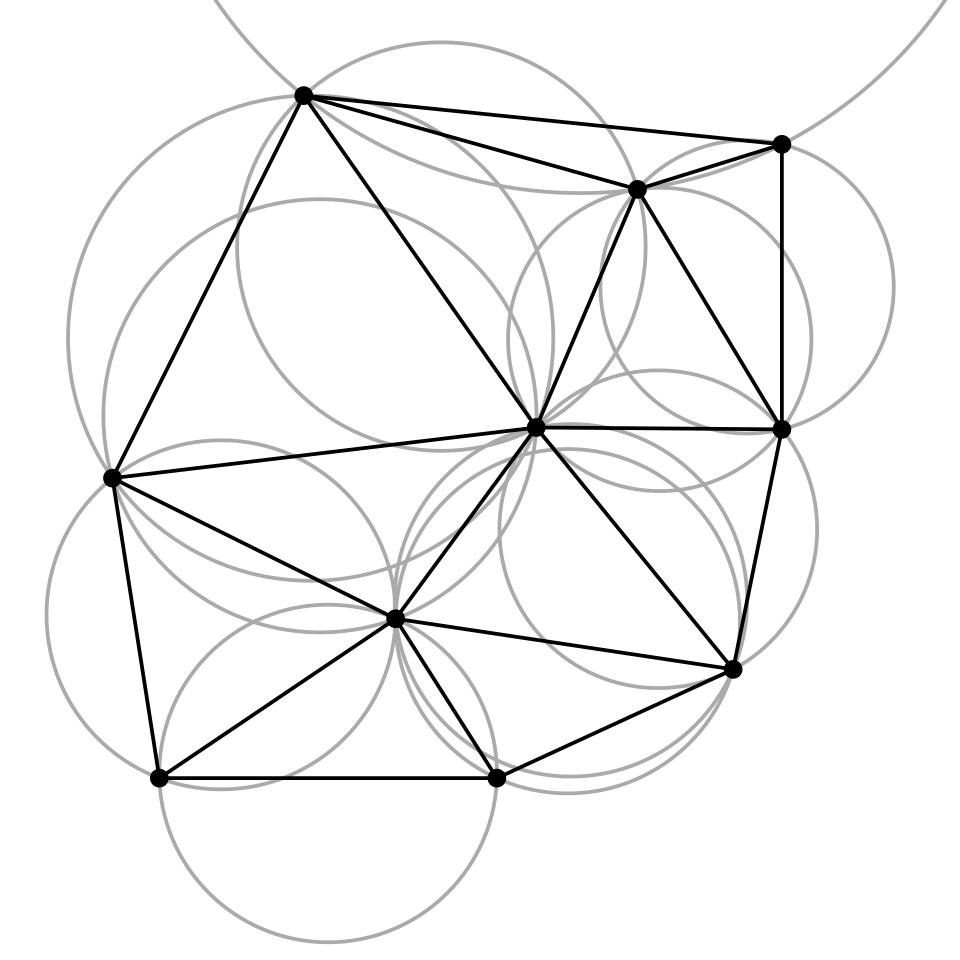
\includegraphics[width=0.3\textwidth]{delaunay_kruznice.png}
    \caption{Princíp reprezentace digitálního modelu terénu pomocí nepravidelné trojúhelníkové sítě (TIN) \parencite{wiki}.}
    \label{fig:princip_dmt}
\end{figure}

\section{Morfometrické analýzy terénu}
Digitální model terénu umožňuje kvantitativní hodnocení geometrických vlastností reliéfu. V rámci této úlohy byly realizovány plošné analýzy sklonu a expozice (orientace) svahu, přičemž výpočet je prováděn nezávisle pro každý trojúhelník triangulační sítě na základě jeho normálového vektoru.

\subsection{Analýza sklonu (Slope)}
Sklon terénu představuje maximální míru změny nadmořské výšky mezi daným elementem a jeho bezprostředním okolím. Podle standardní logiky geografických informačních systémů tento výpočet identifikuje nejprudší klesání ze zkoumaného místa. V případě polyedrického (TIN) modelu je sklon konstantní pro celou plochu konkrétního trojúhelníku a geometricky odpovídá úhlu, který svírá rovina tohoto trojúhelníku s horizontální rovinou $xy$.

Sklon svahu lze primárně vyjadřovat dvěma způsoby: ve stupních (kde hodnoty leží v intervalu od 0 do 90 stupňů) nebo v procentech (tzv. percent rise, což představuje poměr vertikálního převýšení ku horizontální vzdálenosti vynásobený hodnotou 100). 

\begin{figure}[H]
    \centering
    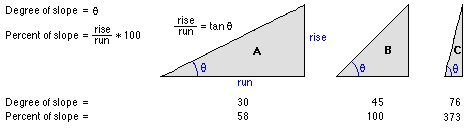
\includegraphics[width=0.8\textwidth]{slope.jpg}
    \caption{Princip vyjádření sklonu terénu ve stupních a v procentech. \parencite{slope}}
\end{figure}

Matematický výpočet vychází z první derivace funkce povrchu $\rho(x,y)$, respektive z vektoru gradientu:
\begin{equation}
    \nabla\rho = \left( \frac{\partial \rho}{\partial x}, \frac{\partial \rho}{\partial y}, -1 \right)
\end{equation}

Velikost samotného sklonu $\alpha$ lze odvodit ze složek gradientu a v naší aplikaci je počítána pomocí následujícího vztahu:
\begin{equation}
    \tan \alpha = \sqrt{\left(\frac{\partial \rho}{\partial x}\right)^2 + \left(\frac{\partial \rho}{\partial y}\right)^2}
\end{equation}

Pro vizualizaci výsledků na modelu je použita spojitá barevná škála nejen v odstínech šedi (viz níže). Důležitým krokem bylo přeškálovat výsledné hodnoty do rozmezí 0-255 pro snadnou vizualizaci. Rovinaté oblasti s minimálním sklonem jsou zobrazeny světlými tóny, zatímco strmější svahy a výrazné terénní zlomy jsou vykresleny úměrně tmavšími odstíny, což umožňuje okamžitou vizuální identifikaci členitosti reliéfu.

\subsection{Analýza expozice (Aspect)}
Expozice (orientace) svahu identifikuje směr nejprudšího klesání, tedy směr maximální míry změny nadmořské výšky od daného elementu k jeho bezprostřednímu okolí. Lze si ji představit jako směr střelky kompasu, ke kterému je analyzovaný svah fyzicky přivrácen. 

Hodnota expozice je měřena ve stupních v rozsahu od 0 do 360. Měření probíhá vždy po směru hodinových ručiček, přičemž hodnota $0^\circ$ (stejně jako $360^\circ$) odpovídá přesnému severu, $90^\circ$ východu, $180^\circ$ jihu a $270^\circ$ západu. Zvláštním případem jsou absolutně rovinaté oblasti s nulovým sklonem. Ty logicky nemají definovanou žádnou orientaci vůči světovým stranám a standardně se jim v systémech přiřazuje hodnota -1.

\begin{figure}[H]
    \centering
    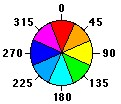
\includegraphics[width=0.3\textwidth]{aspect.jpg}
    \caption{Kategorizace azimutu expozice do směrů světových stran podle kompasu \parencite{aspect}.}
\end{figure}

Matematický výpočet azimutu $A$ vychází ze složek gradientu do horizontální roviny $xy$ a je definován pomocí funkce arkustangens:
\begin{equation}
    A = \arctan\left(\frac{\frac{\partial \rho}{\partial y}}{\frac{\partial \rho}{\partial x}}\right)
\end{equation}

Při kartografické vizualizaci je spojitý rozsah 360 stupňů zpravidla reklasifikován do osmi základních směrových sektorů reprezentujících hlavní světové strany. Každému tomuto intervalu je následně přiřazena unikátní barva. Tento přístup umožňuje snadnou vizuální interpretaci prostorového uspořádání reliéfu, což je klíčové například pro analýzu dopadu slunečního záření nebo modelování odtoku povrchových vod.


\section{Generování a vizualizace vrstevnic}
Vrstevnice jsou izolinie, které propojují body se stejnou hodnotou nadmořské výšky. V digitálním modelu terénu slouží k vizualizaci vertikální členitosti reliéfu a umožňují interpretaci tvarů zemského povrchu z rovinného zobrazení. Proces tvorby vrstevnic v aplikaci vychází z průsečíků horizontálních rovin v definovaných výškových úrovních s hranami polyedrického modelu.

\subsection{Parametry konstrukce vrstevnic}
Při generování vrstevnic jsou klíčové dva parametry: základní interval (Contour Interval) a východisková úroveň (Base Contour). Interval určuje vertikální vzdálenost mezi sousedními vrstevnicemi a přímo ovlivňuje hustotu výsledné kresby. Východisková úroveň definuje nadmořskou výšku, od které se interval začíná odpočítávat (zpravidla se jedná o hodnotu 0). 

Pro zvýšení čitelnosti a přehlednosti výškopisu, zejména v členitém terénu, se využívá rozlišení linií na základní a zvýrazněné. Zvýrazněné vrstevnice jsou vykreslovány s větším krokem (zpravidla pětinásobkem základního intervalu) a jsou graficky odlišeny větší tloušťkou čáry. Toto bxlo ve skriptu docíleno pomocí podmínky \texttt{z \% (self.\_\_dz * 5) == 0}, která testuje, zda je aktuální nadmořská výška bezezbytku dělitelná pětinásobkem kroku \texttt{dz}. Pokud je podmínka splněna, je následně vrstevnice zvýrazněná.

\begin{figure}[H]
    \centering
    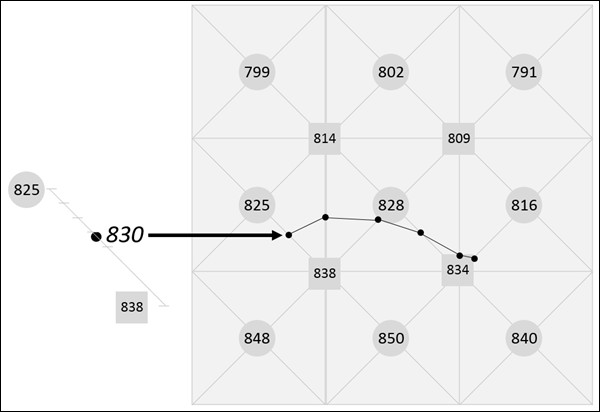
\includegraphics[width=0.7\textwidth]{contour.jpg}
    \caption{Princip generování vrstevnic z digitálního modelu povrchu\parencite{contour}.}
\end{figure}

\subsection{Algoritmus lineární interpolace}
Konstrukce jednotlivých segmentů vrstevnic probíhá pomocí lineární interpolace na hranách trojúhelníků sítě TIN. Předpokládáme, že nadmořská výška se podél hrany mění lineárně. Pro každou hranu definovanou koncovými body $P_1=[x_1, y_1, z_1]$ a $P_2=[x_2, y_2, z_2]$ algoritmus nejprve ověří, zda hledaná výšková úroveň $z$ spadá do intervalu výšek obou bodů. 

V kladném případě je poloha průsečíku $[x, y]$ vypočtena podle následujících vztahů:

\begin{equation}
    x = x_1 + (x_2 - x_1) \cdot \frac{z - z_1}{z_2 - z_1}
\end{equation}

\begin{equation}
    y = y_1 + (y_2 - y_1) \cdot \frac{z - z_1}{z_2 - z_1}
\end{equation}

Vypočtené průsečíky v rámci jednoho trojúhelníku jsou následně propojeny úsečkou, čímž vzniká segment vrstevnice. Výsledná čára je pak složena z těchto na sebe navazujících segmentů napříč celou trojúhelníkovou sítí.

\clearpage
\newpage

\section{Vstupní data a jejich předzpracování}
Základním předpokladem pro tvorbu digitálního modelu terénu je zajištění kvalitních výškových dat. V rámci tohoto projektu byla využita reálná geodetická data poskytovaná Českým úřadem zeměměřickým a katastrálním (ČÚZK). Konkrétně se jedná o data z produktu Digitální model reliéfu 5. generace (DMR 5G), který vznikl metodou leteckého laserového skenování. Pro účely testování a vizualizace byl zvolen výřez reálného území v oblasti Ústí nad Labem. Data jsou distribuována v souřadnicovém systému S-JTSK (Křovákovo zobrazení) ve formátu \texttt{.xyz} \parencite{cuzk}.

\begin{figure}[H]
    \centering
    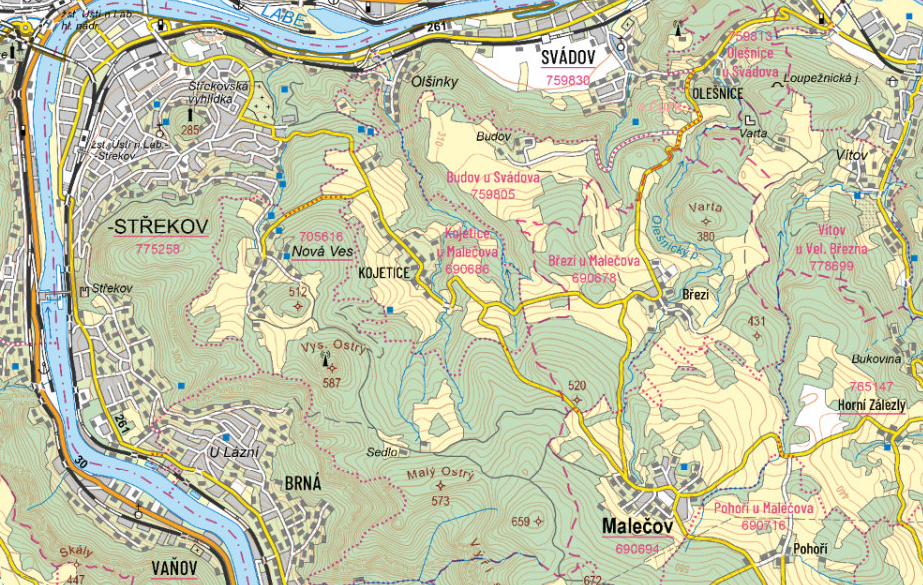
\includegraphics[width=0.8\textwidth]{Misto_dat.png}
    \caption{Vymezení zájmové oblasti v okolí Ústí nad Labem \parencite{cuzk}.}
\end{figure}

\subsection{Redukce bodového mračna}
Původní datové sady z ČÚZK obsahují pro jeden standardní mapový list stovky tisíc až miliony bodů. Zpracování takto masivního mračna bodů v naší aplikaci by vedlo k enormní výpočetní zátěži a případnému zamrznutí programu při konstrukci triangulační sítě. Z tohoto důvodu bylo nutné data před nahráním do aplikace předzpracovat.

K prostorové redukci byl využit open-source software CloudCompare. Byla aplikována metoda náhodného vzorkování (Random Subsampling), pomocí které bylo původní mračno bodů zredukováno na optimální množinu přibližně 300 až 500 bodů. Zredukovaná data byla exportována do standardního textového souboru.

\subsection{Proces načítání a souřadnicová transformace}
Aplikace je uzpůsobena k načítání textových souborů, přičemž algoritmus sekvenčně prochází jednotlivé řádky a extrahuje prostorové souřadnice $[x, y, z]$. Vzhledem k tomu, že vstupní souřadnice v systému S-JTSK dosahují hodnot v řádech stovek tisíců metrů a operují v odlišném kvadrantu, provádí aplikace ihned po načtení souboru automatickou transformaci do lokálního pixelového systému plátna:

\begin{itemize}
    \item \textbf{Výpočet obalového obdélníku (Bounding Box):} Algoritmus vyhledá globální minima a maxima pro osy X a Y, čímž přesně definuje prostorový rozsah načteného území.
    \item \textbf{Změna měřítka (Scale Factor):} Následně je vypočítán poměr pro přepočet reálných souřadnic na pixely tak, aby se model proporčně vešel do okna aplikace. Výpočet zachovává stejné měřítko pro obě osy, aby nedošlo k deformaci reliéfu.
    \item \textbf{Kartografická korekce orientace:} Standardní grafické knihovny umisťují počátek souřadnicové soustavy vlevo nahoru, přičemž hodnoty Y rostou směrem dolů. Pro zachování správné kartografické orientace (kde sever směřuje nahoru) je souřadnice Y při vykreslování transformována. Souřadnice Z zůstává během celého procesu nezměněna, aby nebyly ovlivněny výpočty vrstevnic a sklonu.
\end{itemize}

\section{Implementace bonusových úloh}
V rámci lepší přehlednosti a doplnění kartografické úplnosti byly přídány další bonusové prvky mimo základní zadání. Prostředí aplikace bylo stále upravováno pomocí PyQt6. Těmito prvky byly: \textbf{volba barevných stupnic} a \textbf{automatický popis vrstevnic}.

\begin{small}
\begin{longtable}{|p{15cm}|c|}

\hline
\textbf{Krok} & \textbf{Hodnocení} \\ \hline\hline
\textit{Výběr barevných stupnic při vizualizaci sklonu a expozice.} & \textit{+3b} \\ \hline
\textit{Automatický popis vrstevnic.} & \textit{+3b} \\ \hline
\textbf{Celkem:} & \textbf{+6b} \\ \hline
\end{longtable}
\end{small}
\vspace{2em}

\subsection{Výběr barevných stupnic při vizualizaci sklonu a expozice}
Tato část byla provedena tak, aby si mohl uživatel zvolit jednu z přednastavených barevných schémat pro vizualizaci sklonu či expozice. Uživatel má na výběr vždy ze ctyř stupnic, které vhodně ale odlišně vystihují daný parametr. Nabídku vizualizace je možné zvolit v hlavní liště, do které byly přidány \textit{Dropdown menu} pomocí \texttt{QComboBox}. Tento seznam umožní uživateli vybrat barevné schéma bez nutnosti opětovného přepočtu dat. Bohužel volba zcela vlastních barev a stupnic by sice byla vhodná, avšak náročná na implementaci. 
\subsubsection{Vizualizace expozice}
Pro zobrazení expozice svahů k osmi hlavním světovým stranám byly v kódu předdefinovány čtyři sady barev pomocí specifických kódů barev objektu \texttt{QColor}. Uživatel si může vybrat z následujících možností:

\begin{itemize}
    \item \textbf{Rainbow:} Standardní duhová stupnice.
    \item \textbf{Pastel Rainbow:} Utlumená duhová stupnice.
    \item \textbf{Magma:} Stupnice od tmavých do zlutooranžových barev.
    \item \textbf{Contrast:} Stupnice s výraznými barvami.
\end{itemize}

Pomocí číselného indexu zvolené barevné palety a podmínky \texttt{if/elif} je vybráno barevné schéma, které si uživatel zvolil. Následně pomocí algoritmu je vyhledána příslušná barva odpovídající vypočtenému azimutu. Níže jsou zobrazeny jednotlivé možnosti vizualizace (obrázek 6).
% Pomoc od AI - worflow a syntax jak by měl vypadat subfigure
\begin{figure}[htbp]
    \centering
    
    % první 2
    \begin{subfigure}[b]{0.45\textwidth}
        \centering
        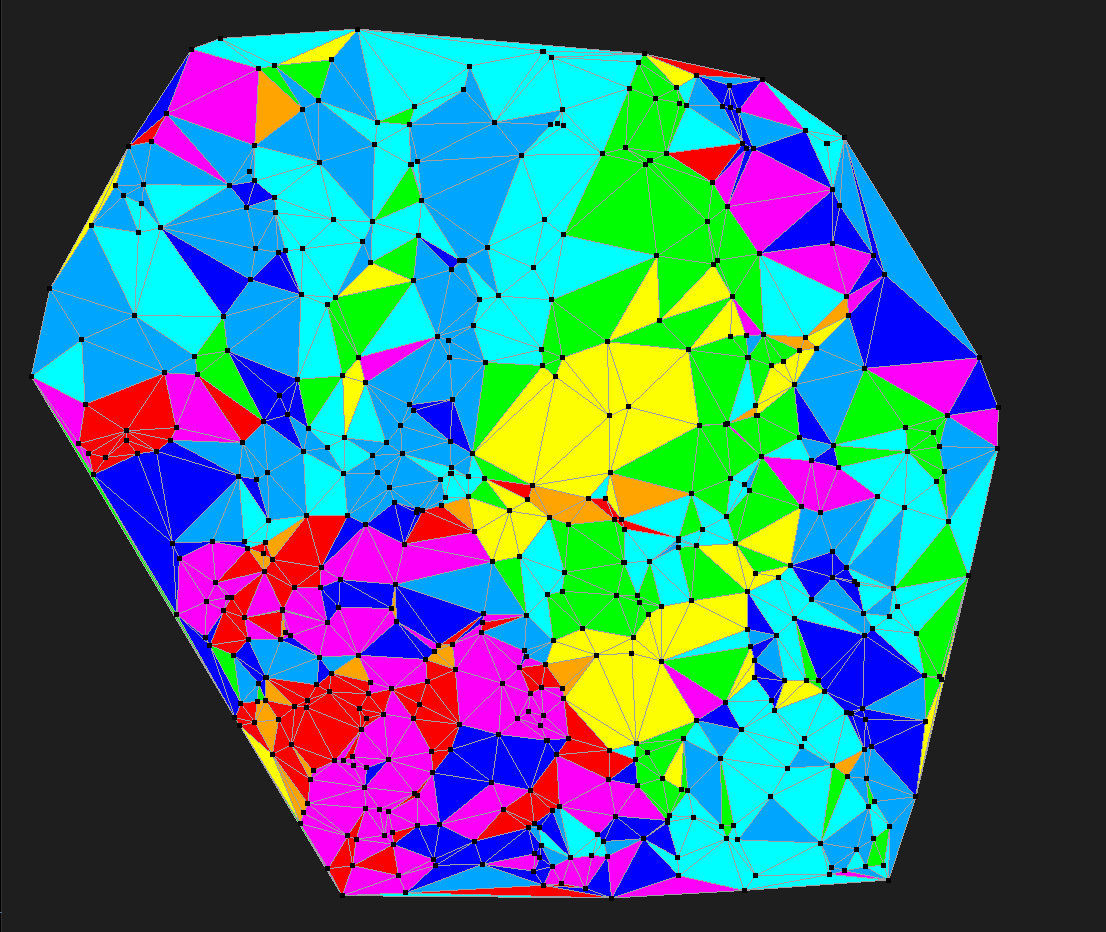
\includegraphics[width=\textwidth]{rainbow.png}
        \caption{Rainbow}
        \label{fig:exp_a}
    \end{subfigure}
    \hfill 
    \begin{subfigure}[b]{0.45\textwidth}
        \centering
        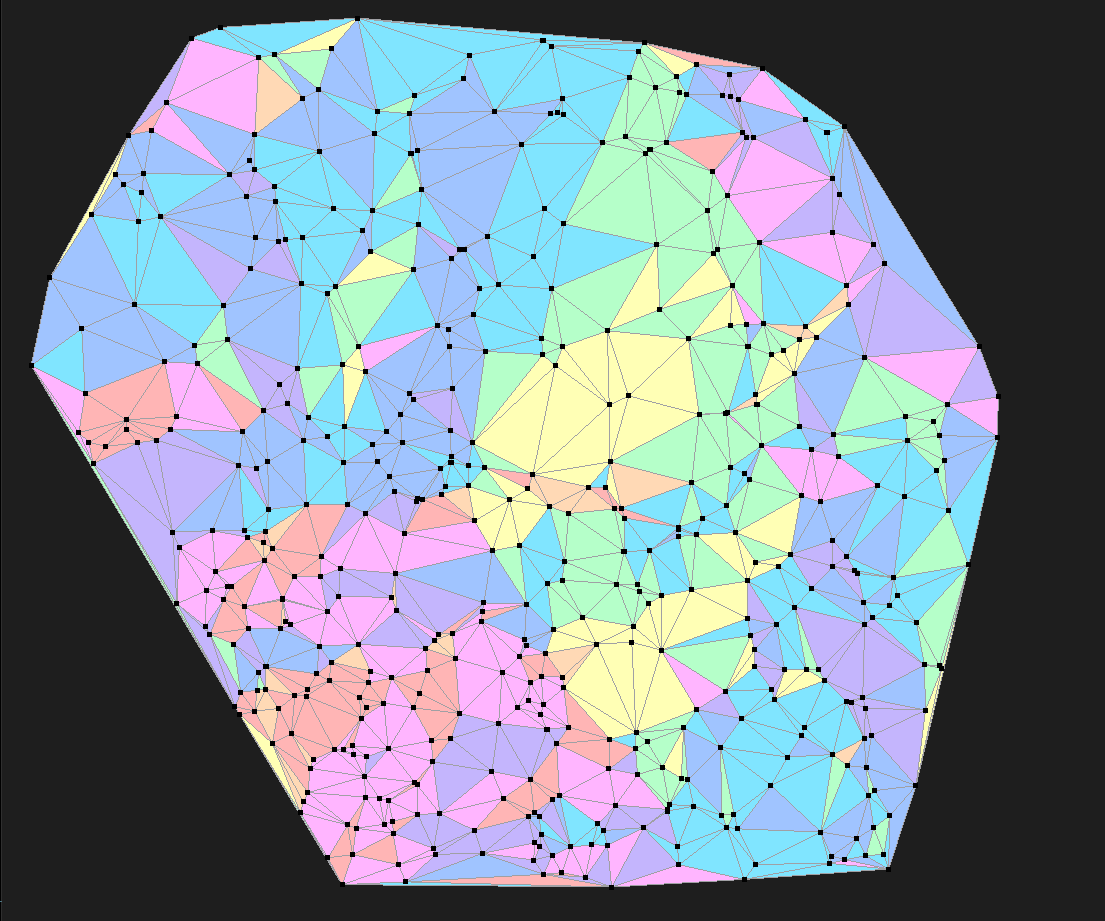
\includegraphics[width=\textwidth]{pastel.png}
        \caption{Pastel Rainbow}
        \label{fig:exp_b}
    \end{subfigure}
    
    \vspace{1em} 
    
    % spodní
    \begin{subfigure}[b]{0.45\textwidth}
        \centering
        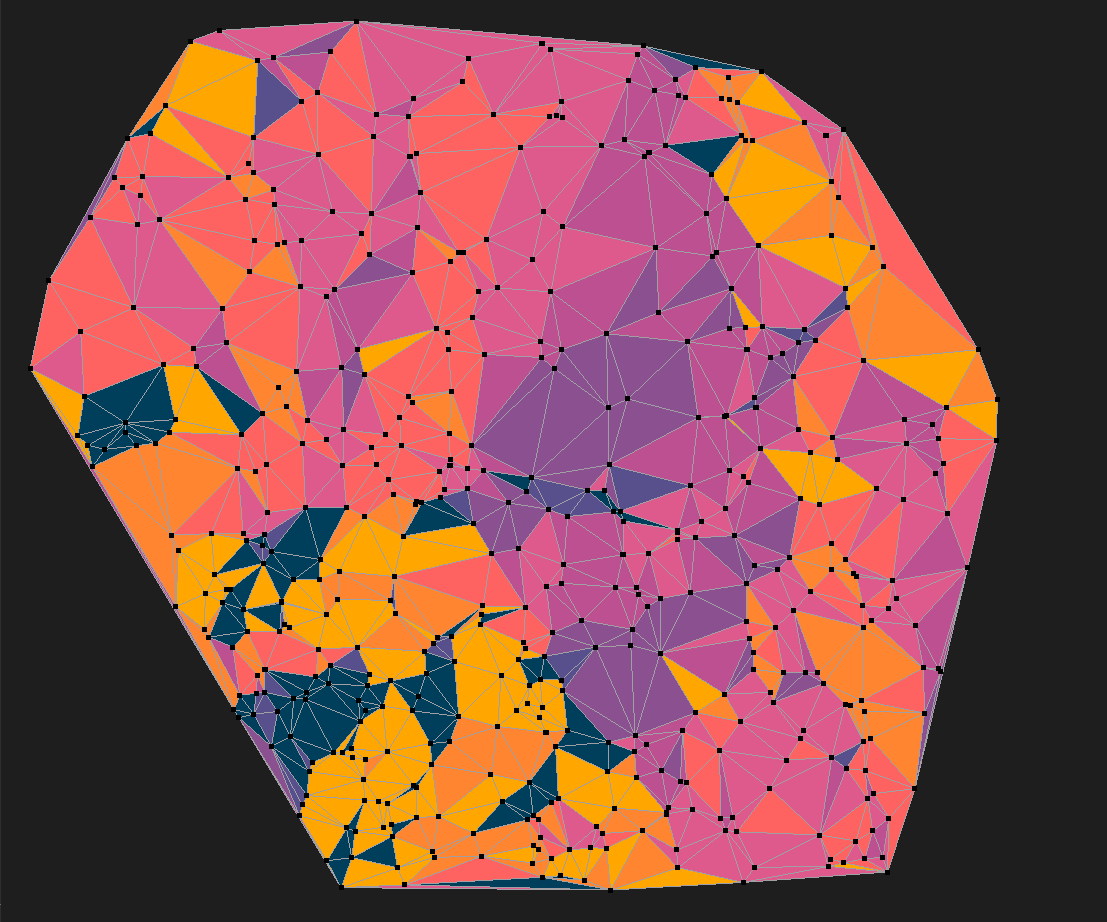
\includegraphics[width=\textwidth]{magma.png}
        \caption{Magma}
        \label{fig:exp_c}
    \end{subfigure}
    \hfill
    \begin{subfigure}[b]{0.45\textwidth}
        \centering
        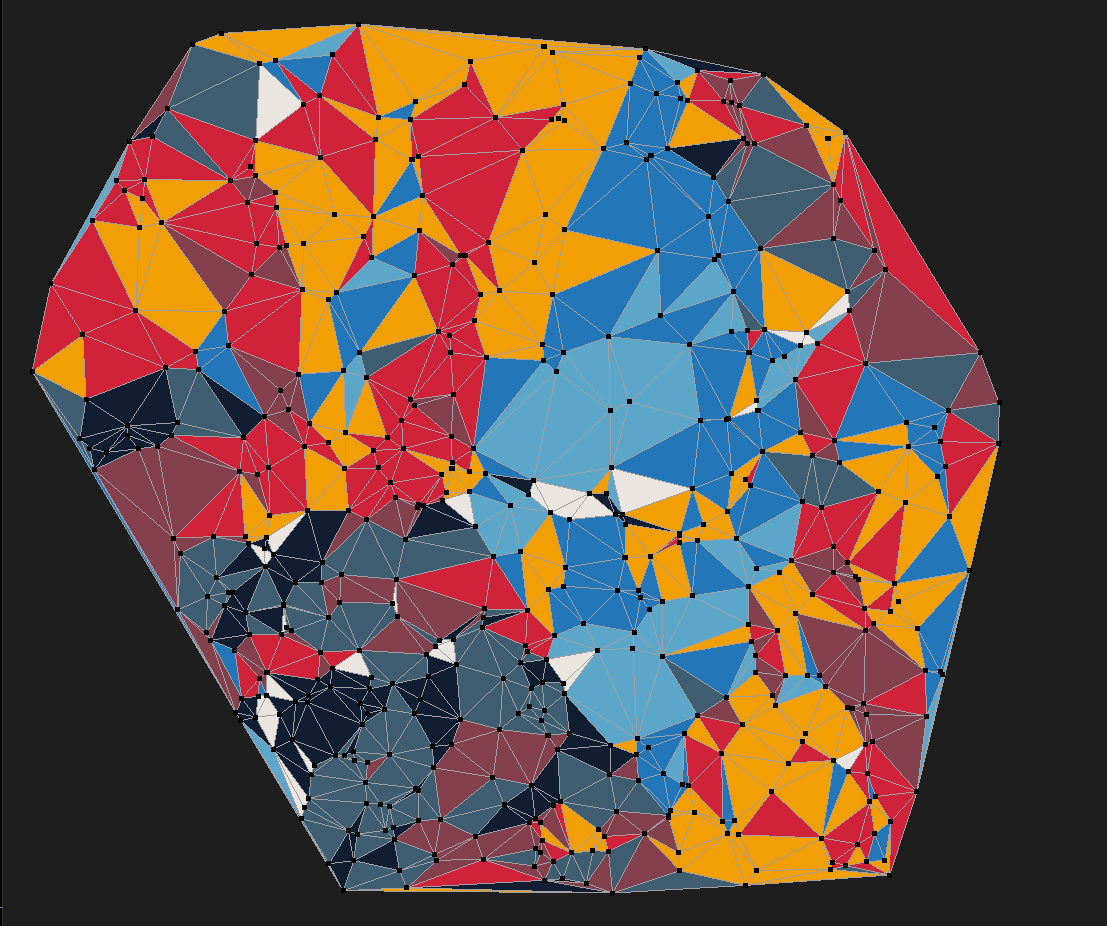
\includegraphics[width=\textwidth]{contrast.png}
        \caption{Contrast}
        \label{fig:exp_d}
    \end{subfigure}

    % popis
    \caption{Zmíněné vizualizace orientace svahu}
    \label{fig:all_exp}
\end{figure}

\clearpage
\newpage

\subsubsection{Vizualizace sklonu}
Na rozdíl od expozice, která využívá 8 směrů, je sklon svahu spojitá veličina. Nebylo tedy využito 8 různých barev, ale byl aplikován plynulý gradient. Jak již bylo zmíněno, bylo nutné hodnoty úhlu přeškálovat na hodnoty 0-255 a provést číselnou inverzi (\texttt{255 -  hodnota}), aby světlé barvy odpovídaly rovinám a naopak. Tyto hodnoty byly dále použity pro barevné zobrazení třídy \texttt{QColor}, která má jako vstupní parametry barevné kanály RGB. Pomocí upravování těchto kanálů je možné zobrazit 4 nabízené barevné škály:

\begin{itemize}
    \item \textbf{Greyscale:} Stupně šedi.
    \item \textbf{Yellow-Red:} Roviny jsou zobrazeny žlutě, strmé svahy červeně.
    \item \textbf{White-Blue:} Přechod z bílé do tmavě modré.
    \item \textbf{White-Purple:} Přechod z bílé do tmavě růžové.
\end{itemize}

Stejně jako u vizualizace orientace sklonu je výběr i této barevné škály tvořen podmínkou \texttt{if/elif}. Pomocí algoritmu je pak přiřazen příslušný odstín podle sklonu plošky. Na obrázku 7 jsou zobrazeny jednotlivé barevné vizualizace.

% Pomoc od AI - worflow a syntax jak by měl vypadat subfigure
\begin{figure}[htbp]
    \centering
    
    % první 2
    \begin{subfigure}[b]{0.45\textwidth}
        \centering
        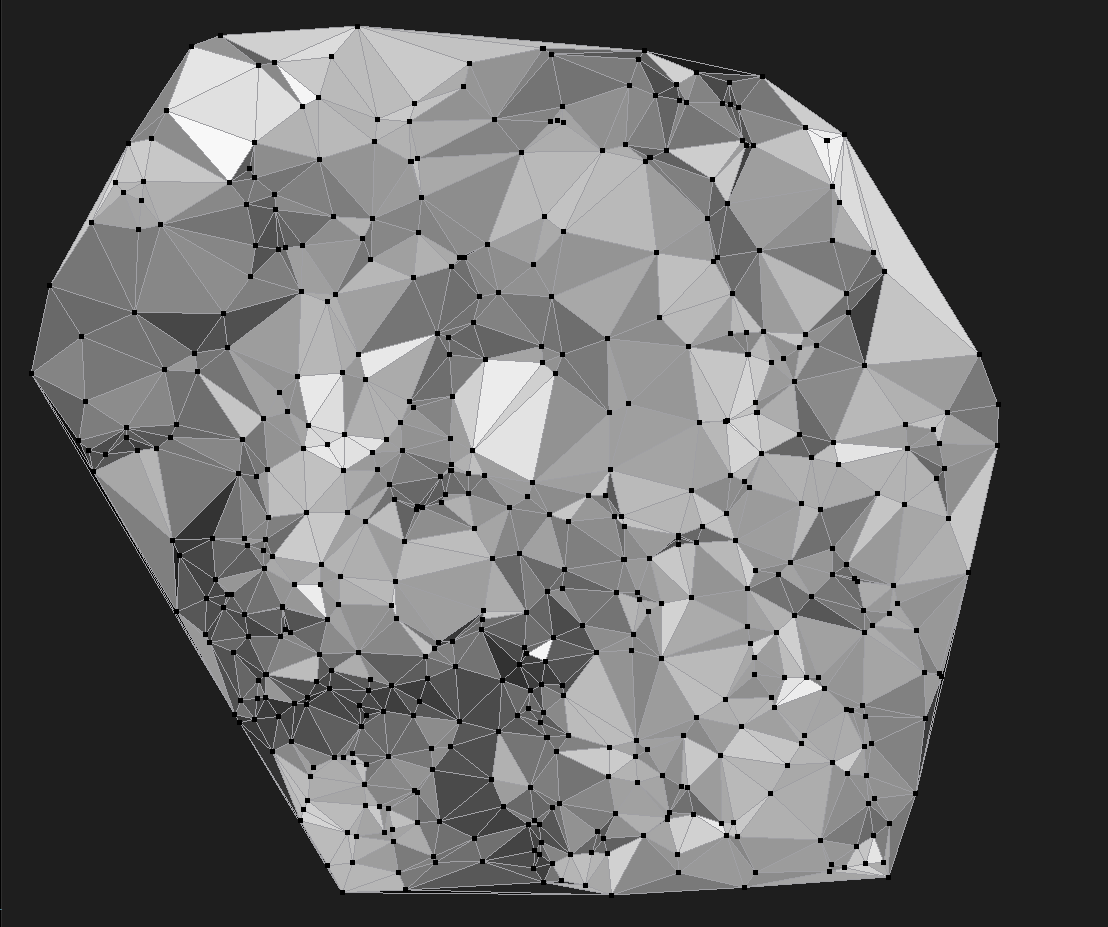
\includegraphics[width=\textwidth]{grayscale.png}
        \caption{Grayscale}
        \label{fig:slope_a}
    \end{subfigure}
    \hfill 
    \begin{subfigure}[b]{0.45\textwidth}
        \centering
        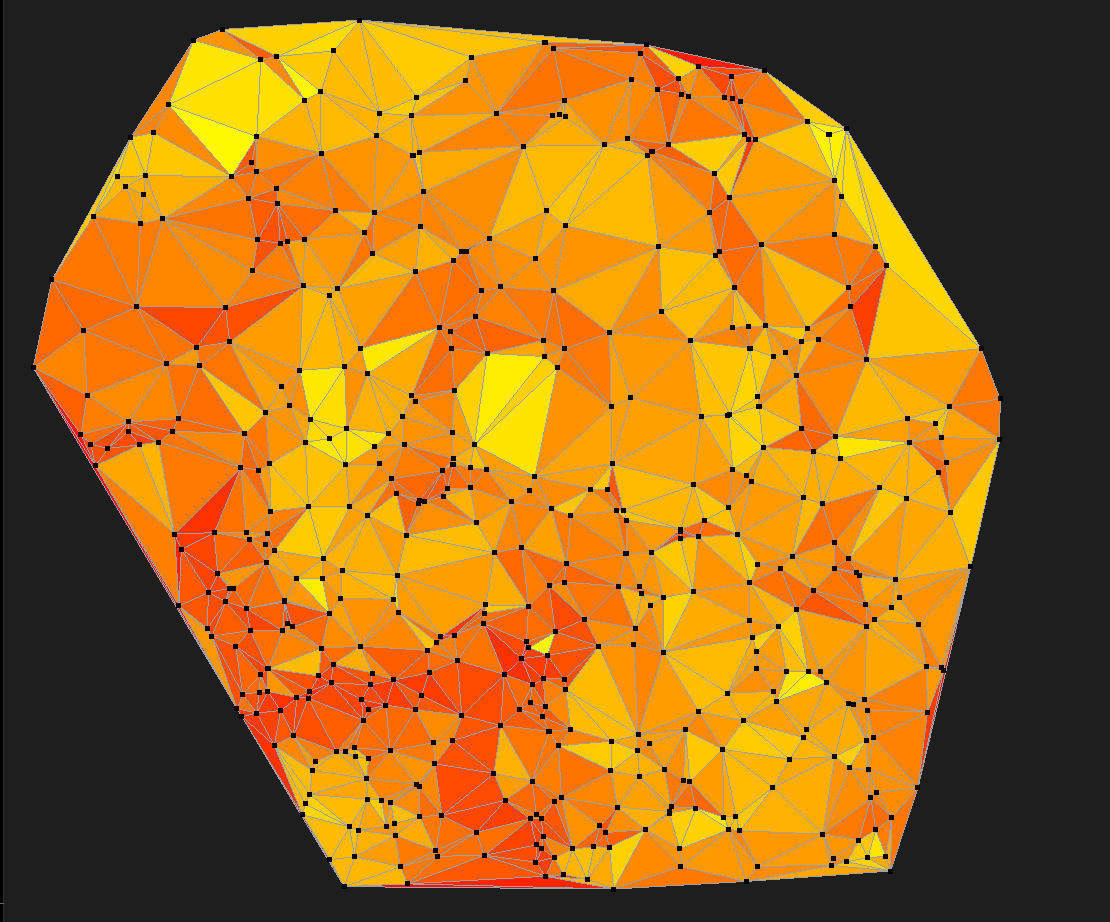
\includegraphics[width=\textwidth]{yellow_red.png}
        \caption{Yellow-Red}
        \label{fig:slope_b}
    \end{subfigure}
    
    \vspace{1em} 
    
    % spodní 2
    \begin{subfigure}[b]{0.45\textwidth}
        \centering
        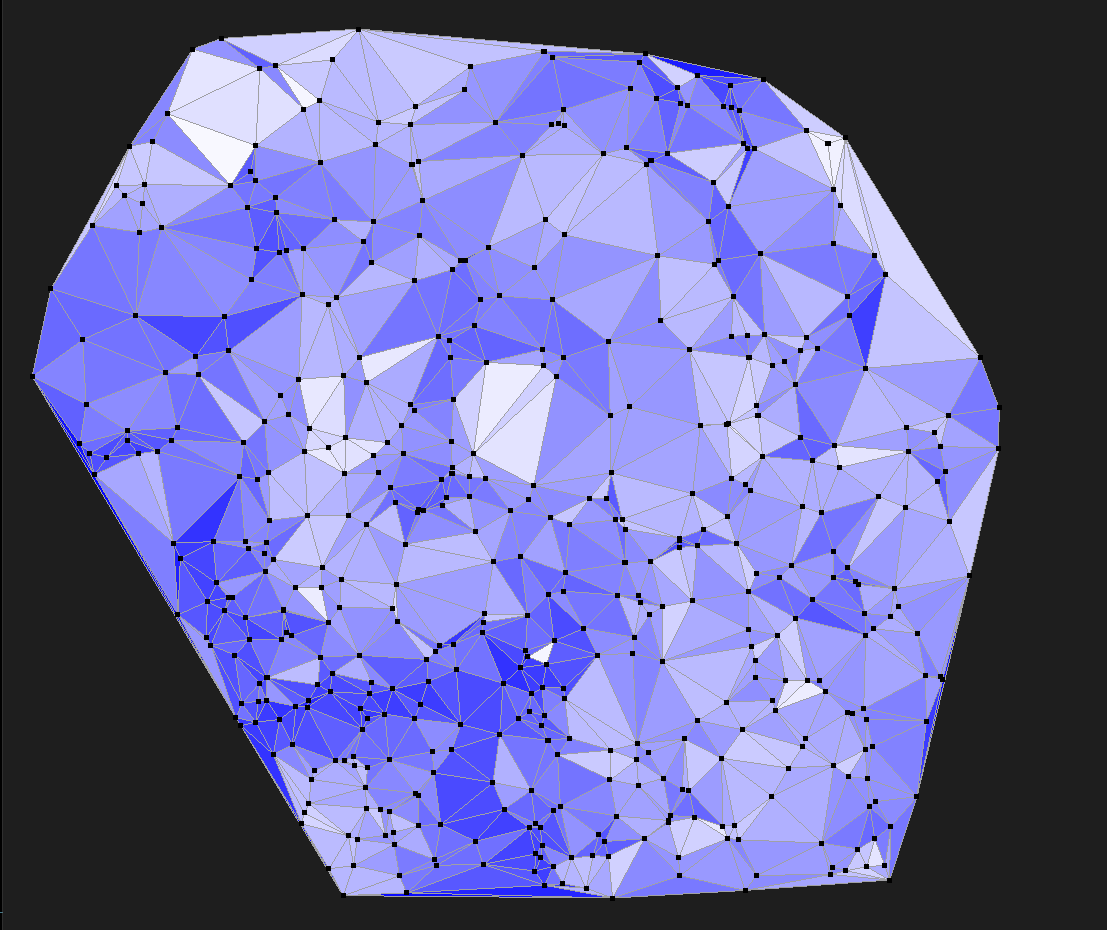
\includegraphics[width=\textwidth]{white_blue.png}
        \caption{White-Blue}
        \label{fig:slope_c}
    \end{subfigure}
    \hfill
    \begin{subfigure}[b]{0.45\textwidth}
        \centering
        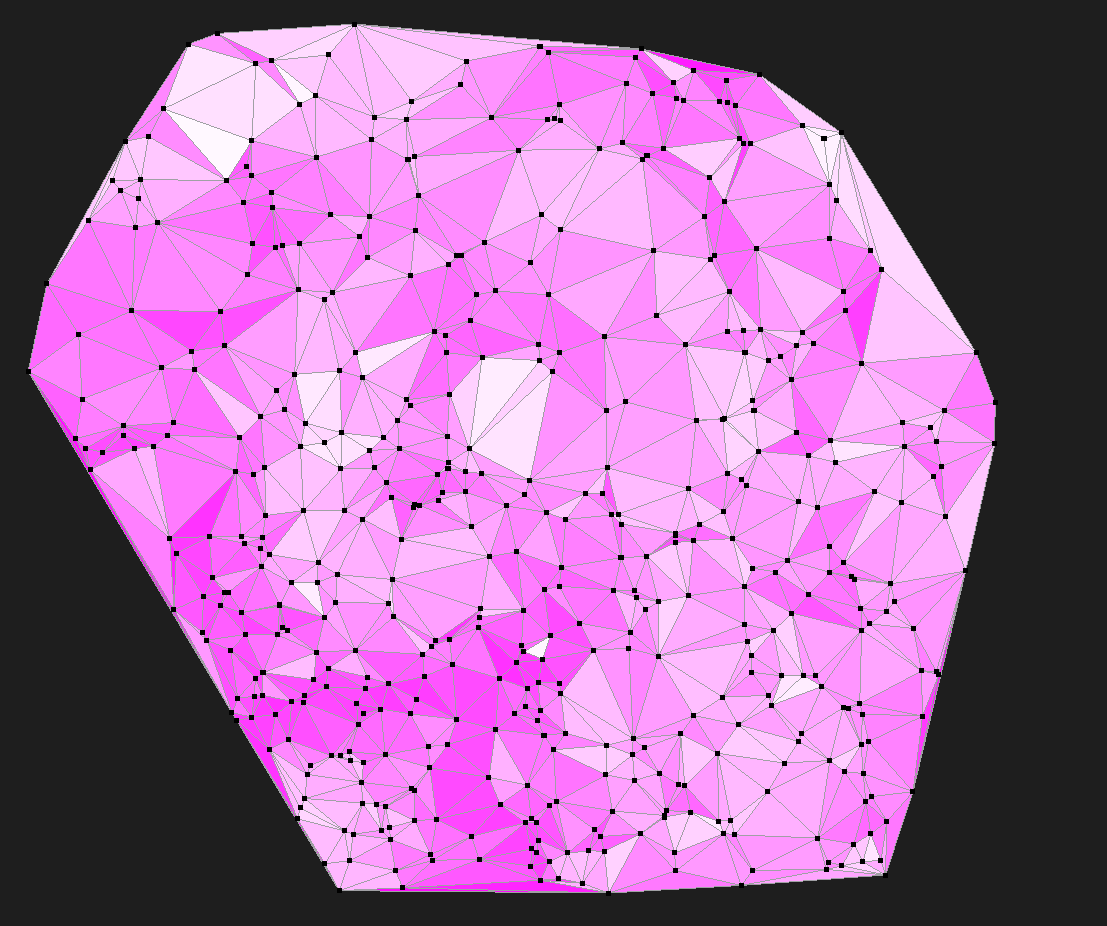
\includegraphics[width=\textwidth]{white_purple.png}
        \caption{White-Purple}
        \label{fig:slope_d}
    \end{subfigure}

    % popis
    \caption{Zmíněné vizualizace sklonu svahu}
    \label{fig:all_slope}
\end{figure}

\subsection{Automatický popis vrstevnic.}
Jak již bylo zmíněno výše, vykreslení vrstvenic rozlišuje základní a zvýrazněné vrstevnice. Pro lepší kartografickou orientaci byly doplněny i popisy vrstevnic. 

Důležitým faktorem však musela stále být přehlednost celkového výsledku, nebylo tedy možné přiřadit popisy ke každé vrstevnici v každé ploše. Tento problém byl vyřešenen přidáním "počítadla", které kontroluje počet vykreslených vrstevnic. Pro toto počítadlo byla dále přidána podmínka \texttt{if counter \% x == 0}, kde \texttt{x} je zvolený parametr - tedy pokud výsledek zbytku po dělění \texttt{x} je 0. Pokud je tedy podmínka splněna, je vypočítán střed dané vrstevnice a vložen popis s odpovídající nadmořskou výškou. Každým opakováním cyklu \texttt{for} je přidána hodnota 1 do počítadla (buďto k zvýrazněné či základní).

Z důvodu udržení přehlednosti byl zvolen parametr \texttt{x} pro zvýrazněné vrstevnice $x = 20$, tedy každá 20. vykreslená zvýrazněná vrstevnice má popis. Popis u zvýrazněných vrstevnic je vykreslen stejnou barvou a větší velikostí písma než u základních vrstevnic. Naopak pro základní vrstevnice, kterých je mnohem více, byl zvolen $x = 35$ a menší font písma. Na obrázku 8 lze pozorovat vykreslené popisy vrstevnic podle našich pravidel. 

\begin{figure}[H]
    \centering
    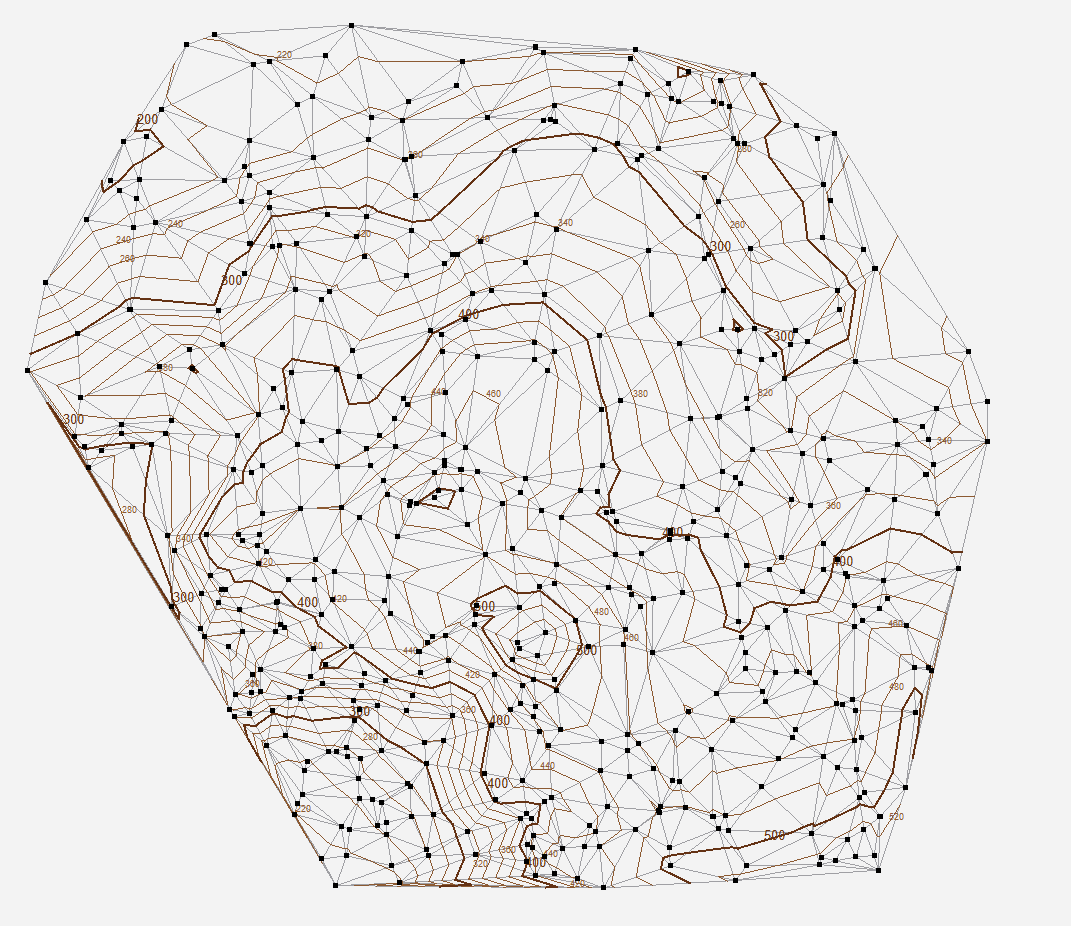
\includegraphics[width=0.8\textwidth]{vrstevnice_popis.png}
    \caption{Vykreslení vrstevnic s popisy.}
\end{figure}

\clearpage
\newpage

\section{Kartografické hodnocení algoritmu}
Tato část bude postupně popisovat výhody a nevýhody algoritmu z hlediska kartografické správnosti. Některé problémy algoritmu se objevily při použití vstupních dat, ale pro některé případy bylo nutné vytvořit vzorová data, na kterých je lépe zachycený daný jev. Pro všechny případy budou přiloženy i ukázky.

\subsection{Výhody a silné stránky algoritmu}
Delaunay triangulace (DT) patíří mezi jeden z nejefektivnějších způsobů reprezentace nepravidelné trojúhelníkové sítě. Mezi její hlavní výhody patří:

\begin{itemize}
    \item \textbf{Trojúhelníková optimalizace:} Algoritmus tvoří trojúhelníky, které se co nejvíce podobají rovnostranným. To minimalizuje vznik úzkých ploch unvnitř dat. Dále zajišťuje plynulý chod a tvar vrstevnic.
    \item \textbf{Hustota dat a jejich věrnost:} Algoritmus dokáže pracovat s proměnlivou hustotou bodů. V rovinatých terénech jsou trojúhelníky větší, zatímco ve složitějších terénech je TIN hustší. Jelikož algoritmus pracuje s přesnými daty a interpolu je je, zachovává 100\% přesnost naměřených dat. Jedná se tedý o věrnou interpolaci povrchu.
\end{itemize}

DT je vhodná na přirozené terény bez ostrých hran, svahu a v našem případě i bze nekonvexních terénech. Obrázek 8 krásně vystihuje výše zmíněné výhody algoritmu

\subsection{Slabiny a limity algoritmu}
Při vuzualizaci určitých terénních tvarů naráží DT na své matematické limity. Tyto situace jsou rozepsány dále.

\subsubsection{Úzké trojúhelníky na okraji dat}
Jelikož algoritmus vytváří pro každý bod trojúhelník, znamená to, že se to děje i pro okajové body. Nastvává tedy situace, ve které se vykreslí úzké plochy s velice hustými vrstevnicemi. Tato situace se objevila v našich datech v jižní části území (obrázek 9). Vrtevnice v těchto plochách vypadají nepřirozeně a neodráží reálný povrch lokality.

\begin{figure}[H]
    \centering
    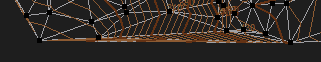
\includegraphics[width=0.8\textwidth]{uzke_trojuhelniky.png}
    \caption{Situace úzkých trojúhelníku v jižní části lokality.}
\end{figure}

\subsubsection{Věrnost dat}
Přestože byla věrnost dat výhodou, lze se na tuto vlastnosti dívat i jako na nevýhodu. Jelikož se jedná o interpolační algoritmus a propojuje pouze reélná data, nelze od něho očekávat extrapolaci. Z toho důvodu lze v některých oblastech pozorovat nepřirozeně vypadající či nevyhlazené vrstevnice. Dále při absenci některých dat lze nastat situace špatné reprezentace povrchu. Na obrázku 10 jsou zobrazeny podobné modelové situace, pro které byly vytvořeny soubory s modelovými daty \texttt{test\_spravny\_vrchol.txt} a \texttt{test\_spatny\_vrchol.txt}. Nalevo je do dat přidán vrchol \texttt{z = 600}, zatímco vpravo je stejný situace, ale bez přidaného vrcholu. Z obrázku je vidět, že alboritmus jakoby seříznul kopec, jelikož mu chyběly příslušná data o povrchu. Tato situace se může objevit i opačně, například u údolí či závrtů.

\begin{figure}[htbp]
    \centering
    
    % první 2
    \begin{subfigure}[b]{0.45\textwidth}
        \centering
        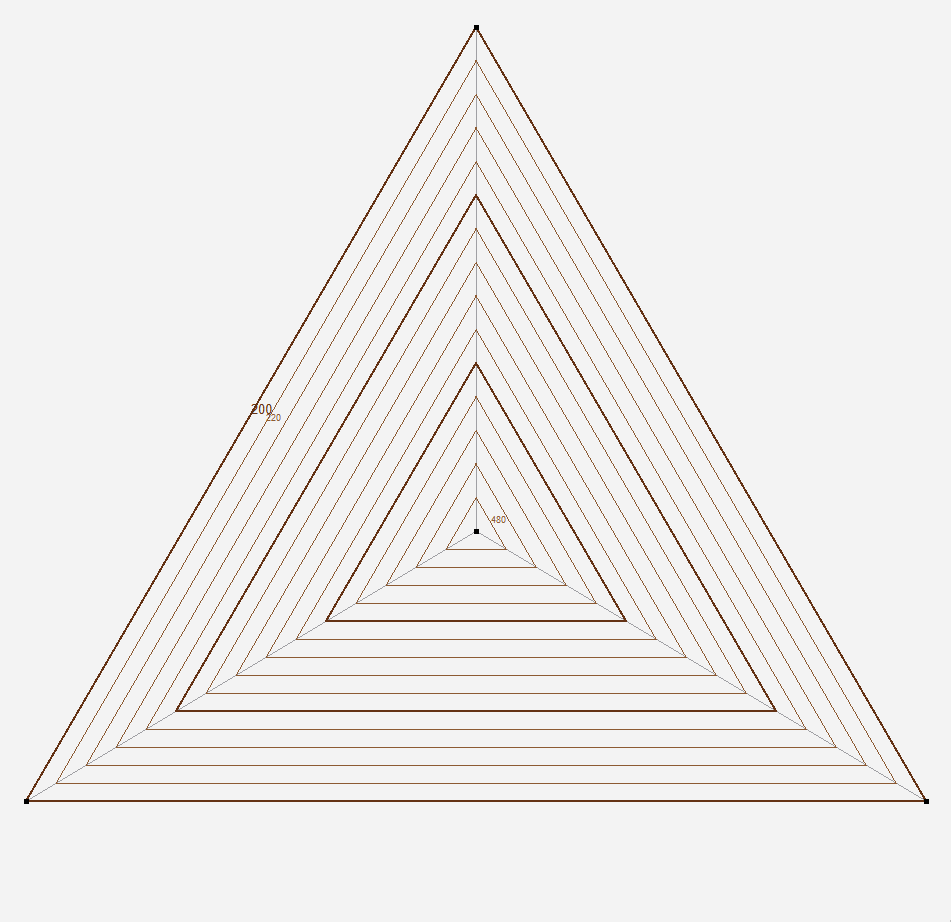
\includegraphics[width=\textwidth]{test_spravny_vrchol.png}
        \caption{Správná situace}
        \label{fig:slope_a}
    \end{subfigure}
    \hfill 
    \begin{subfigure}[b]{0.45\textwidth}
        \centering
        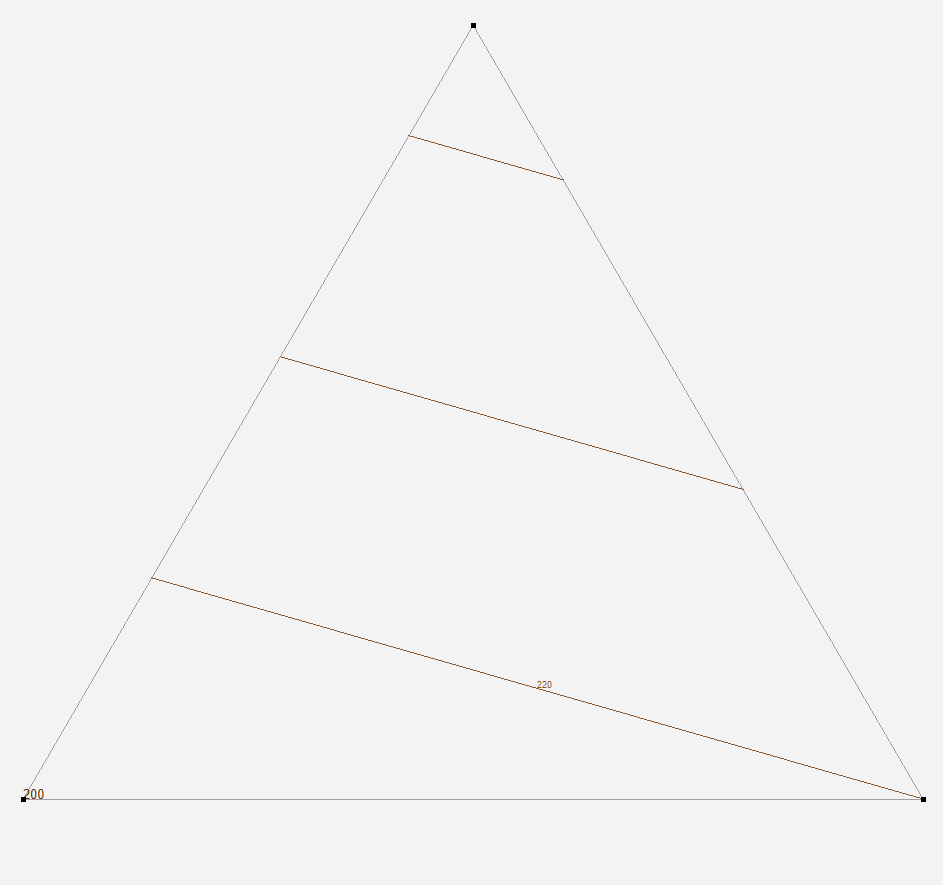
\includegraphics[width=\textwidth]{test_spatny_vrchol.png}  
        \caption{Špatná situace}
        \label{fig:slope_b}
    \end{subfigure}

    % popis
    \caption{Ukázka věrnosti dat algoritmu}
\end{figure}

\subsubsection{Absence povinných hran}
Jelikož DT funguje na hledání nejideálnějších trojúhelníků, ke každému bodu, nezná tam například hřbetnice či údolí/řeky. Kvůli této vlastnosti neví algoritmus, že se zde objevuje určitá povinná hrana, kterou nesmí překročit či přetvořit. Tedy namísto, aby vytvořil trojúhelníky vedle souběžně s hlavní hranou, ignoruje tuto hranu a tudíž i daný krajinný jev.

V případě našich dat je problém zřejmý. Mimo řeku, která teče v levé části dat jsou zde i jiné povinné hrany, např. hřbetnice, silnice či jiné říčky. Všechny tyto krajinné jevy algoritmus ignoruje a přetváří tak interpretaci krajiny.


\begin{figure}[htbp]
    \centering
    
    % první 2
    \begin{subfigure}[b]{0.75\textwidth}
        \centering
        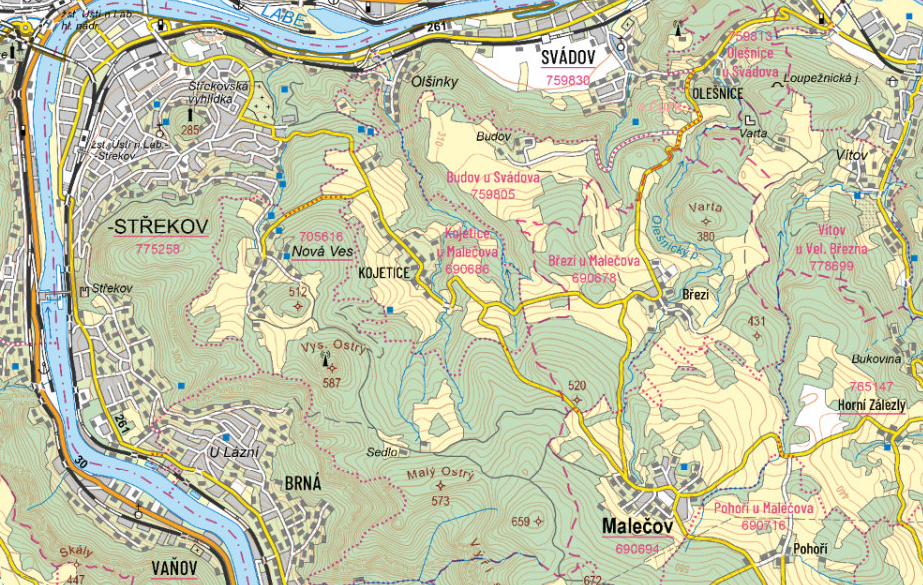
\includegraphics[width=\textwidth]{Misto_dat.png}
        \caption{Reálný povrch}
        \label{fig:slope_a}
    \end{subfigure}
    
    \vspace{1em} 
    
    \begin{subfigure}[b]{0.75\textwidth}
        \centering
        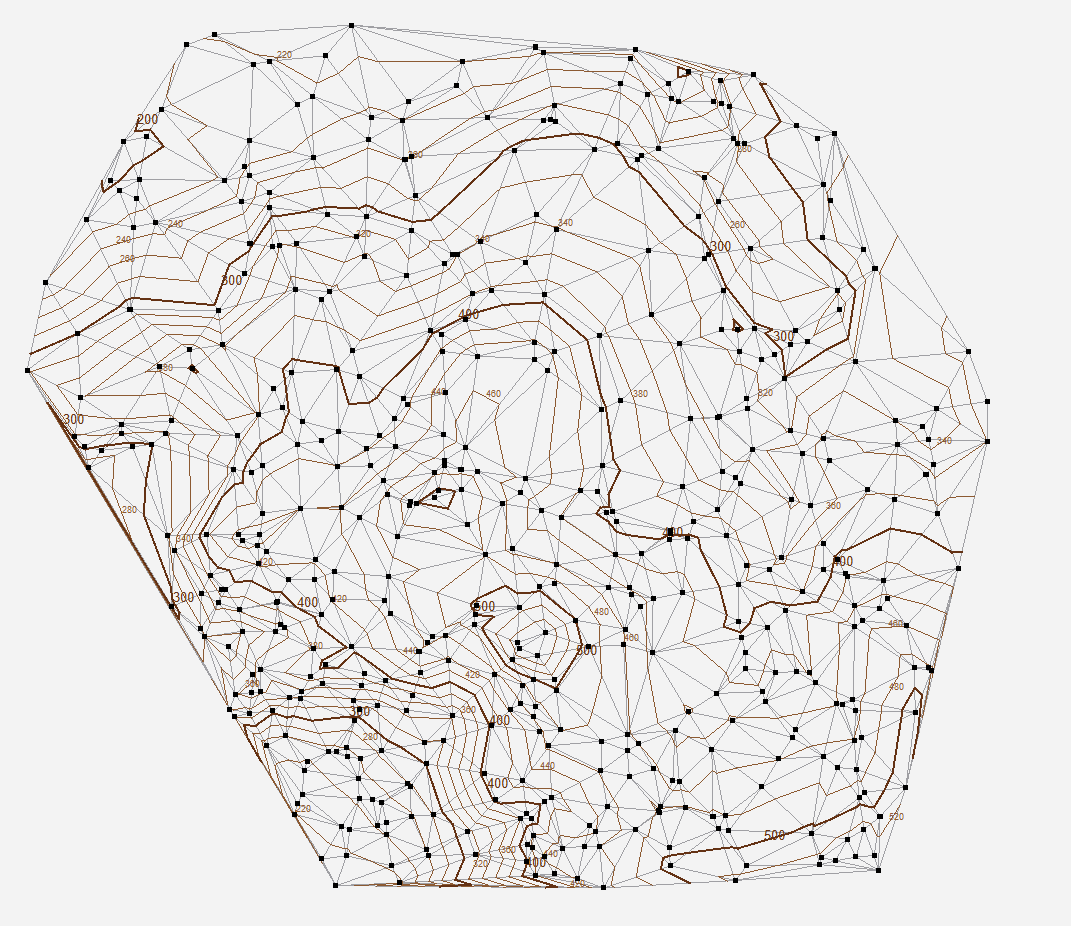
\includegraphics[width=\textwidth]{vrstevnice_popis.png}
        \caption{Výsledek algoritmu}
        \label{fig:slope_c}
    \end{subfigure}

    % popis
    \caption{Ukázka absence povinných hran}
\end{figure}

\newpage

Přes uvedené slabiny je vytvořený algopritmus vysoce funkční, zvládá správně relativně správně interpolovat a reprezentovat reálný povrch. Pomocí bonusové vizualizace (sklon, orientace) je možné snadněji data interpretovat a výsledek je lehce čitelný.

\section{Třídy a jejich metody}
Pro správný chod aplikace bylo využito objektově orientovaného programování, přičemž architektura je rozdělena do několika specifických tříd. Třída \texttt{MainForm.py} má na starosti veškerou logiku uživatelského rozhraní, napojení tlačítek a načítání souborů. 

Třída \texttt{Draw.py} spravuje samotné plátno a zajišťuje grafické vykreslování všech prvků. 

Třída \texttt{Algorithms.py} obsahuje veškeré interpolační a analytické metody. 

Pro uchování specifických datových struktur byly vytvořeny pomocné třídy \texttt{QPoint3DF.py}, \texttt{Edge.py} a \texttt{Triangle.py}.


\subsection{Třída MainForm}
\begin{itemize}
    \item \textbf{setupUi} – Inicializuje a rozmisťuje grafické prvky v okně aplikace, tvoří horní lištu (včetně nástrojů \texttt{QComboBox} pro volbu barev) a propojuje tlačítka s příslušnými funkcemi.
    \item \textbf{createDTClick} – Načte body z plátna a spouští algoritmus pro tvorbu Delaunayovy triangulace.
    \item \textbf{createContourLinesClick} – Spouští výpočet pro generování vrstevnic na základě uživatelem zadaných parametrů.
    \item \textbf{analyzeSlopeClick / analyzeExpositionClick} – Spouští analýzy sklonu či expozice nad vytvořeným modelem.
    \item \textbf{viewDTClick / viewContoursClick / viewSlopeClick / viewAspectClick} – Zajišťují přepínání vykreslení jednotlivých vrstev analýz.
    \item \textbf{openFileClick} – Otevírá okno pro výběr \texttt{.txt} souboru, načítá z něj data, vypočítává min-max box a provádí kartografickou transformaci (změna měřítka a inverze osy Y) pro správné vykreslení na plátno.
    \item \textbf{settingsClick} – Otevírá vedlejší dialogové okno pro zadání parametrů vrstevnic ($Z_{min}$, $Z_{max}$, $dz$).
    \item \textbf{clearResultsClick / clearAllClick} – Čistí mapové plátno; první metoda vymaže pouze výsledky analýz, druhá vymaže kompletně vše.
    \item \textbf{changeAspectColorsClick / changeSlopeColorsClick} – Získávají index zvolené barevné škály z dropdown menu pro změnu vizualizace.
\end{itemize}

\subsection{Třída Algorithms}
\begin{itemize}
    \item \textbf{createDT} – Hlavní funkce realizující 2D Delaunayovu triangulaci nad vstupní množinou bodů metodou inkrementální konstrukce.
    \item \textbf{findDelaunayPoint} – Vyhledává optimální bod z množiny pro vytvoření nového Delaunayovského trojúhelníku na základě testování podmínky pázdné opsané kružnice.
    \item \textbf{getPointLinePosition} – Testuje vzájemnou polohu bodu a přímky (half-plane test) pro určení poloroviny, v níž se bod nachází.
    \item \textbf{getNearestPoint} – Vyhledá k zadanému inicializačnímu bodu nejbližší bod z množiny pro založení první hrany.
    \item \textbf{get2LinesAngle} – Vypočítá úhel mezi dvěma směry.
    \item \textbf{updateAEL} – Zajišťuje správu seznamu aktivních hran (\textit{Active Edge List}); řeší přidávání a odebírání hran na základě jejich orientace.
    \item \textbf{createContourLines} – Prochází vygenerovanou trojúhelníkovou síť a generuje vrstevnice.
    \item \textbf{createContourLineSegment / getContourPoint} – Využívají lineární interpolaci pro výpočet přesných souřadnic průsečíku vrstevnice s hranou trojúhelníku.
    \item \textbf{analyzeDTM} – Funkce, která projde celou triangulaci a pro každý trojúhelník zavolá výpočet sklonu a expozice.
    \item \textbf{getSlope / getAspect} – Získají normálový vektor roviny trojúhelníku a vypočítají maximální sklon (v radiánech) a azimut expozice ($0-360^\circ$).
\end{itemize}

\subsection{Třída Draw}
\begin{itemize}
    \item \textbf{mousePressEvent} – Zachytává kliknutí uživatele, získává souřadnice kurzoru a generuje bod s náhodnou výškou Z pro interaktivní tvorbu modelu.
    \item \textbf{paintEvent} – Metoda vykreslování; vizualizuje trojúhelníkovou síť, vrstevnice (včetně grafického odlišení a popisu) a zbarvené plochy pro analýzy sklonu a expozice.
    \item \textbf{setAspectScheme / setSlopeScheme} – Ukládají index zvoleného grafického schématu vybraného uživatelem v liště.
    \item \textbf{clearResults / clearAll} – Resetují ukládací seznamy uvnitř plátna pro vymazání plátna.
\end{itemize}

\subsection{Pomocné datové třídy}
\begin{itemize}
    \item \textbf{QPoint3DF} – Rozšiřuje standardní \texttt{QPointF} o uložení třetí souřadnice Z (nadmořské výšky).
    \item \textbf{Edge} – Reprezentuje hranu trojúhelníka; obsahuje metodu pro změnu orientace a porovnávání hran.
    \item \textbf{Triangle} –  Uchovává body, polygon a vypočtené hodnoty sklonu a expozice.
    \item \textbf{Settings} – Definuje dialogové okno pro nastavení parametrů vrstevnic.
\end{itemize}

\section{Závěr}
Pro tento úkol byl vytvořen algoritmus, který vytváří nepravidelnou trojúhelníkovou síť na základě principu 2D Delaunay triangulace. Aplikace byla vytvořena v prostředí QT a doplněna v prostředí programovacího jazyka Python. 

V rámci aplikace si může uživatel vytvořit vlastní modelové území s náhodnými hodnotami výšky \texttt{z} nebo si může importovat vlastní \texttt{.txt} soubor se souřadnicemi. Pomocí nástrojů v hlavní nabídce aplikace je možné analyzovat dané body - \textbf{tvorba DT}, \textbf{interpolace vrstevnic}, \textbf{výpočet a vizualizace sklonu} a \textbf{orientace svahu}. Pro snadnější orientaci byla aplikace doplněna o výběr barevných stupnic pro vizualizaci a také o automatický popis vrstevnic a jejich rozlišení na základní a zvýrazněné. Uživatel si dále může vybrat základní interval vrstevnic pro podrobnější analýzu.

Přestože algoritmus pracuje výborně, vyskytují se zde určité nedostatky, které jsou pro tento algoritmus limitující. Jako problematická místa se jeví okrajové body datového souboru, nekompletní data či ostré a nekonvexní lokality, zejm. převisy, kaňony atp. Z hlediska uživatelského rozhraní není možné přibližovat a oddalovat na vybrané lokality, což se jeví jako lehká nevýhoda. Obdobně není možné posouvat s mapou v rámci většího území.

\printbibliography[title=Zdroje]

\end{document}

